\documentclass[letter]{beamer}
%removed: handout (ignores "animations")

\usepackage[utf8]{inputenc}
\usepackage{graphicx}
\usepackage{minted}

\usetheme{AnnArbor}
%\usetheme{CambridgeUS}
\usecolortheme{beaver}

\title[IIC2333] % (optional, only for long titles)
{09 - Capa de Aplicación}
\subtitle{IIC2333 - Sistemas Operativos y Redes}
\author[C.Ruz] % (optional, for multiple authors)
{Cristian Ruz -- {\tt cruz@ing.puc.cl}\footnote{Material preparado con aporte del profesor Carlos Buil Aranda} }
\institute[PUC] % (optional)
{
  Departamento de Ciencia de la Computación\\
  Pontificia Universidad Católica de Chile
}
\date[2/2015] % (optional)
{Semestre 2-2015}
\subject{I}

\AtBeginSection[]
{
  \begin{frame}
    \frametitle{Contenidos}
    \tableofcontents[currentsection]
  \end{frame}
}

\begin{document}

%---------------------------------------------------------------------
\frame{\titlepage}


%---------------------------------------------------------------------
\begin{frame}
\frametitle{Contenidos}
%\tableofcontents[currentsection]
\tableofcontents
\end{frame}


%---------------------------------------------------------------------
\section{Protocolos de Aplicación}

\begin{frame}
  \frametitle{¿Y las aplicaciones?}
  
  Hasta aquí todo ha sido: ¿cómo enviar datos?
  \begin{itemize}
    \item ¿Enviar bits?: Capa Física
    \item ¿Enviar frames en un enlace?: Capa de Enlace
    \item ¿Mover paquetes de dirección origen a dirección de destino?: Capa de Red
    \item ¿Transmitir un mensaje completo desde nodo origen a nodo destino?: Capa de Transporte
  \end{itemize}
  ¿Y qué hacer con los mensajes? \onslide<2->{{\bf ¡Capa de Aplicación!}}
  
\end{frame}
%---------------------------------------------------------------------
\begin{frame}
  \frametitle{Capa de Aplicación}
  
  Procesos en distintos nodos que intentan comunicarse
  \begin{itemize}
    \item Reglas de comunicación
    \item Comunicación interprocesos
      \begin{itemize}
        \item Pero procesos en distintos {\em hosts}
      \end{itemize}
    \item Aquí se construyen las aplicaciones
  \end{itemize}

\end{frame}

%---------------------------------------------------------------------
\begin{frame}
  \frametitle{Capa de Aplicación}

  Algunos protocolos que funcionan en capa de aplicación:
  \begin{itemize}
    \item DNS, Domain Name System
    \item HTTP, Hypertext Transfer Protocol
    \item FTP, File Transfer Protocol
    \item SSH, Secure Shell
    \item TELNET, Remote Shell
    \item SMTP, Simple Mail Transfer Protocol
    \item POP, Post-Office Protocol
    \item IMAP, Internet Message Access Protocol
    \item NTP, Network Time Protocol
    \item IRC, Internet Relay Chat
    \item LDAP, Lightweight Directory Access Protocol
  \end{itemize}
  Protocolos utilizan servicio de capa de transporte: sockets vía TCP ó UDP
\end{frame}


\begin{frame}
  \frametitle{Arquitecturas}

  ¿Cómo comunicar los procesos?
  
  Dos modelos:
  \begin{itemize}
    \item Cliente-Servidor
      \begin{itemize}
        \item Clásico. Servidor escucha, cliente inicia la comunicación
        \item Servidor debe escuchar en un puerto conocido por el cliente
      \end{itemize}
    \item Peer-to-Peer
      \begin{itemize}
        \item No hay roles específicos de servidor
        \item Sistema decentralizado
        \item Conexiones intermitentes
      \end{itemize}
  \end{itemize}
  

\end{frame}

%---------------------------------------------------------------------
\section{HTTP}

\begin{frame}
  \frametitle{HTTP: HyperText Transfer Protocol}

  Básicamente un sistema de archivos remoto
  \begin{itemize}
    \item Modelo cliente-servidor
    \item Cliente HTTP: solicita y recibe archivos
      \begin{itemize}
        \item Opcionalmente podría parsearlos e interpretarlos localmente
      \end{itemize}
    \item Servidor HTTP: recibe solicitudes y envía archivos
  \end{itemize}
  
  \begin{center}
    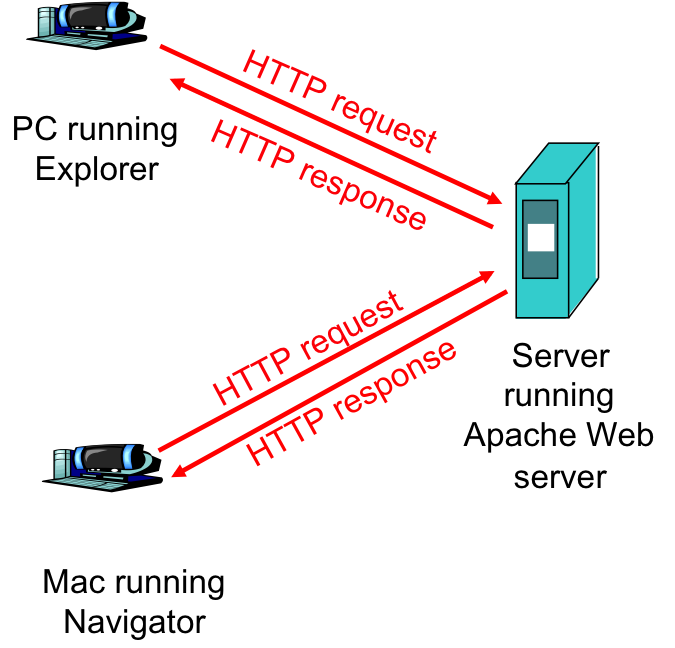
\includegraphics[width=6cm]{figs/09-http.png}
  \end{center}

\end{frame}


%---------------------------------------------------------------------
\begin{frame}
  \frametitle{HTTP: HyperText Transfer Protocol}

  Protocolo sin estado ({\em stateless})
  \begin{itemize}
    \item Cliente crea socket TCP al puerto 80 del servidor
    \item Servidor acepta conexión TCP desde el cliente
    \item Cliente y servidr intercambian mensaje HTTP
    \item Cliente cierra la conexión
    \item Es posible informar que se desea mantener la conexión abierta: HTTP persistente
  \end{itemize}
  Al no tener estado, no se recuerda conexiones anteriores del cliente
  \begin{itemize}
    \item Pero hay mecanismos para mantener un estado en el cliente: {\em cookies}
  \end{itemize}
  Dos tipos de solicitudes
  \begin{itemize}
    \item HTTP Request
    \item HTTP Response
  \end{itemize}
\end{frame}
%---------------------------------------------------------------------
\begin{frame}
  \frametitle{HTTP Request}
  
  Mensajes HTTP se transmiten en formato ASCII (otros protocolos utilizan un formato binario)
  
  \begin{center}
    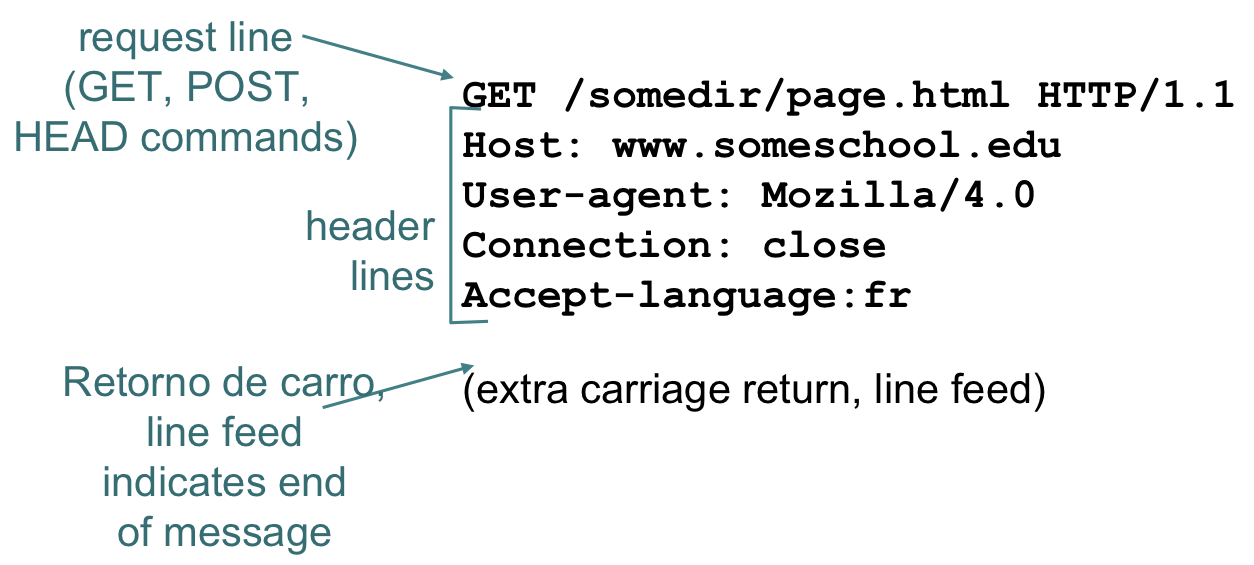
\includegraphics[width=8cm]{figs/09-http-request.png}
  \end{center}

  
\end{frame}
%---------------------------------------------------------------------
\begin{frame}
  \frametitle{HTTP Request}
  
  \begin{center}
    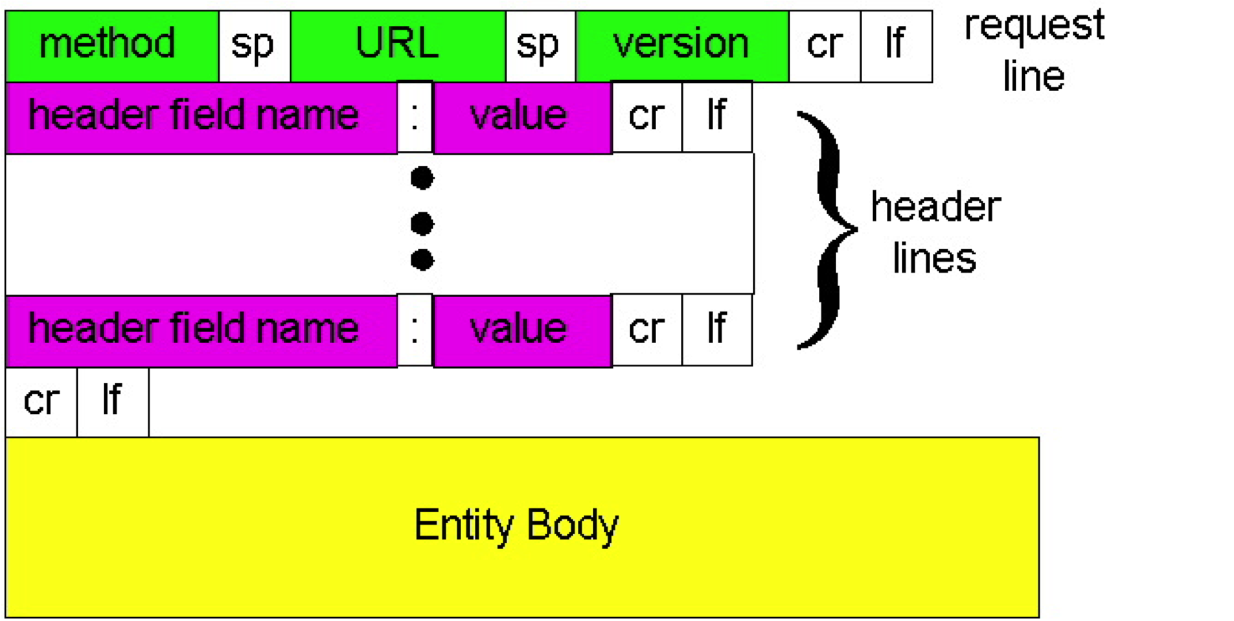
\includegraphics[width=10cm]{figs/09-http-request-2.png}
  \end{center}

  
\end{frame}

%---------------------------------------------------------------------
\begin{frame}
  \frametitle{HTTP Response}
  
  \begin{center}
    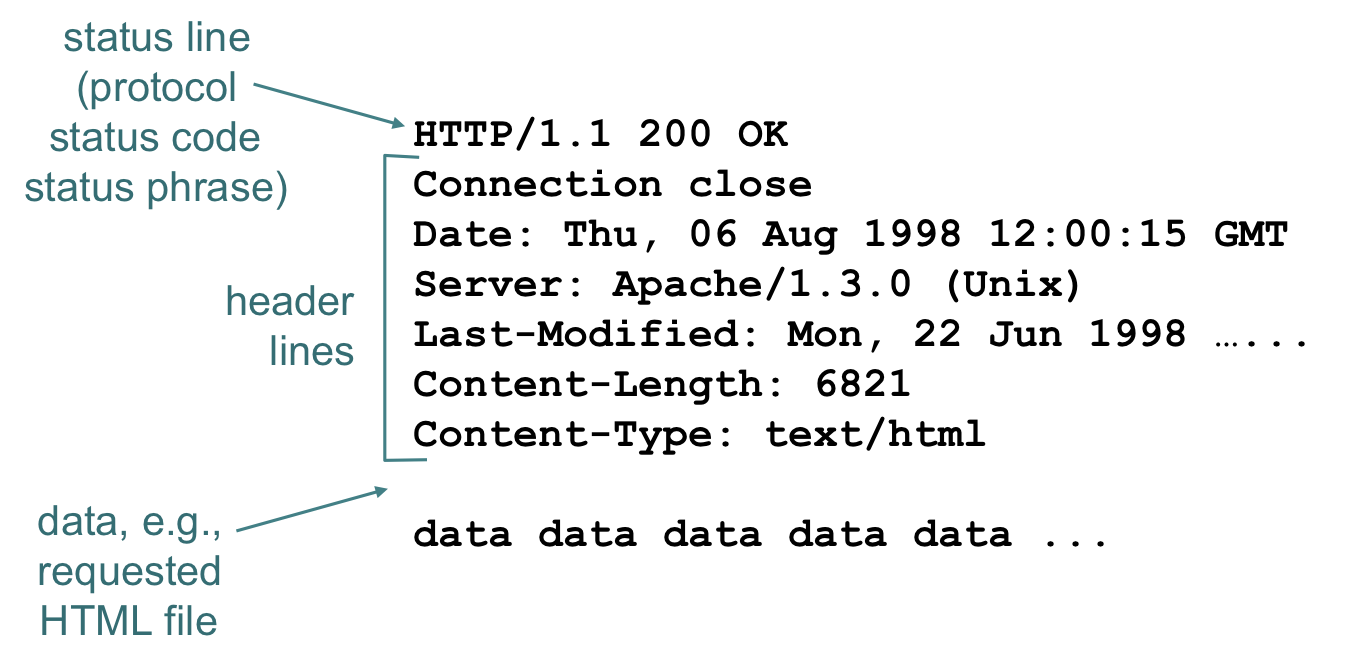
\includegraphics[width=10cm]{figs/09-http-response.png}
  \end{center}
  
\end{frame}


%---------------------------------------------------------------------
\begin{frame}
  \frametitle{HTTP Codes}

  Códigos HTTP indican tipo de respuesta a la solicitud.
  
  \begin{itemize}
    \item 1xx. Mensaje de información.
    \item 2xx. Mensaje de éxito
      \begin{itemize}
        \item 200 OK
        \item 206 Partial Content
      \end{itemize}
    \item 3xx. Mensaje de redirección
      \begin{itemize}
        \item 301 Moved Permanently
        \item 307 Temporary Redirect
      \end{itemize}
    \item 4xx. Mensaje de error del cliente
      \begin{itemize}
        \item 400 Bad Request
        \item 403 Forbidden
        \item 404 Not Found
        \item 405 Method Not Allowed
      \end{itemize}
    \item 5xx. Mensaje de error del servidor
      \begin{itemize}
        \item 500 Internal Server Error
        \item 501 Not Implemented
        \item 502 Bad Gateway
        \item 503 Server Not Available
      \end{itemize}
  \end{itemize}

\end{frame}

%---------------------------------------------------------------------
\section{DNS}

\begin{frame}
  \frametitle{DNS: Domain Name System}

  Una base de datos distribuida
  \begin{itemize}
    \item Almacenamiento de pares $\langle \text{nombre}, \text{dirección IP} \rangle$
    \item Arquitectura cliente/servidor jerárquica
      \begin{itemize}
        \item Servidores se conocen como servidores de nombres
        \item Organización jerárquica permite crear {\em dominios}
        \item Organización jerárquica permite balancear carga
      \end{itemize}
  \end{itemize}
\end{frame}
%---------------------------------------------------------------------
\begin{frame}
  \frametitle{DNS: Domain Name System}

  Organización jerárquica
  \begin{center}
    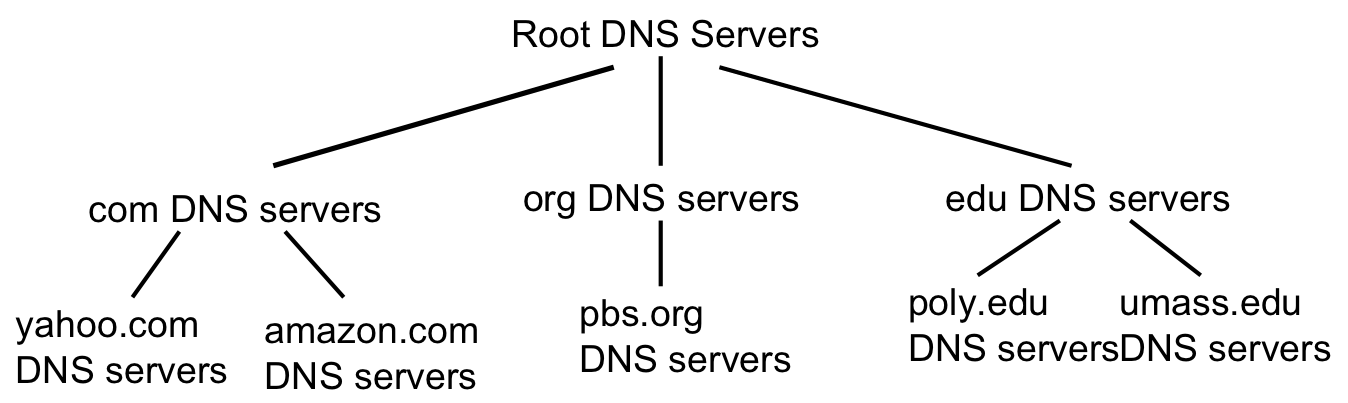
\includegraphics[width=10cm]{figs/09-dns-arbol.png}
  \end{center}
  
\end{frame}

%---------------------------------------------------------------------
\begin{frame}
  \frametitle{DNS: Domain Name System}
  \framesubtitle{Servidores raíz, TLD, autoritativos}
  
  Servidores almacenan {\em mapping}s 
  \begin{itemize}
    \item Si un servidor no conoce un {\em mapping}, lo consulta a un servidor superior en la jerarquía
    \item Eventualmente puede llegar a un servidor raíz
    \item Servidor raíz conocen ubicación de servidores TLD
      \begin{itemize}
        \item gTLD: General Top-Level Domain. {\tt .com}, {\tt .org}, {\tt .edu} 
        \item ccTLD: Country-Code Top-Level Domain. {\tt .cl}, {\tt .nl}, {\tt .es}, {\tt .au}
      \end{itemize}
    \item 13 servidores raíz en el mundo: A,B,C,D,E,F,G,H,I,J,K,L,M
      \begin{itemize}
        \item Con múltiples instancias de cada uno (dos de ellos replicados en Chile)
        \item {\tt http://www.root-servers.org}
      \end{itemize}
    \item Servidores que administran el mapping son {\em servidores autoritativos}
      \begin{itemize}
        \item Servidores autoritativos administran el mapping (al nivel de institución)
        \item Servidores no-autoritativos mantienen temporalmente el mapping
      \end{itemize}
  \end{itemize}

\end{frame}

%---------------------------------------------------------------------
\begin{frame}
  \frametitle{DNS: Domain Name System}
  \framesubtitle{Ejemplo}
  Host en dominio {\tt ing.puc.cl} desea contactar {\tt www.amazon.com}
  
  Consulta iterativa
  \begin{center}
    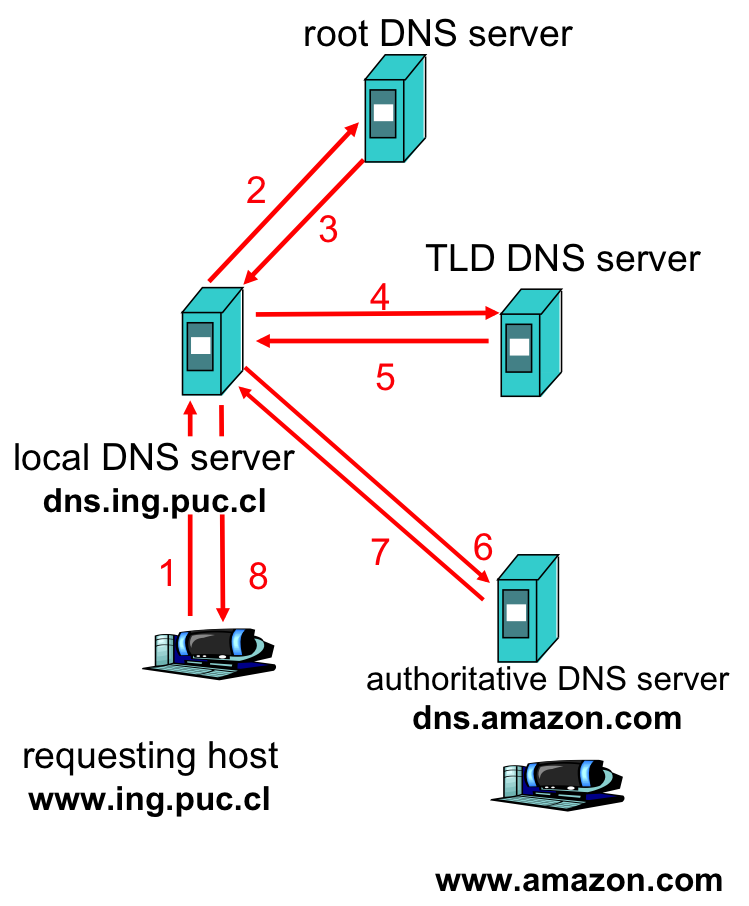
\includegraphics[width=5cm]{figs/09-dns-example.png}
  \end{center}


\end{frame}
%---------------------------------------------------------------------
\begin{frame}
  \frametitle{DNS: Domain Name System}
  \framesubtitle{Ejemplo}

  Host en dominio {\tt ing.puc.cl} desea contactar {\tt www.yahoo.com}
  
  Consulta recursiva
  \begin{center}
    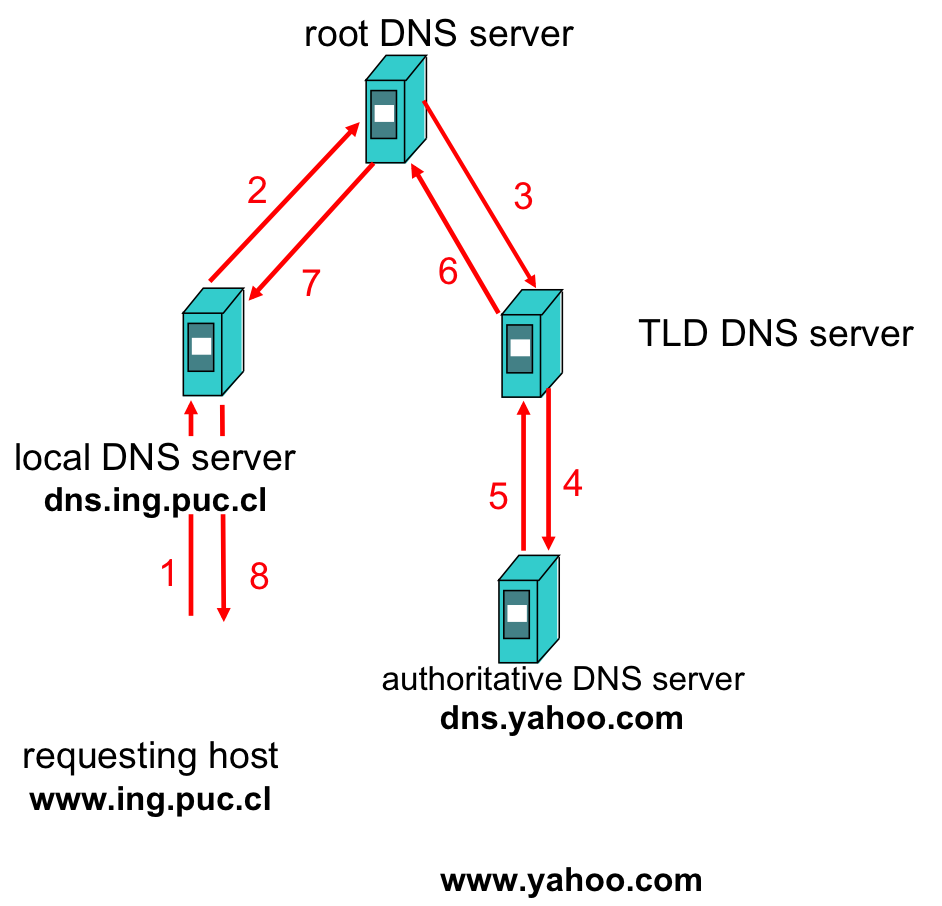
\includegraphics[width=5cm]{figs/09-dns-example-2.png}
  \end{center}


\end{frame}
%---------------------------------------------------------------------
\begin{frame}
  \frametitle{DNS: Domain Name System}
  \framesubtitle{Caching}

  Al resolver un mapping, éste es almacenado en los servidores
  \begin{itemize}
    \item Caching de respuestas permite reducir el tráfico
    \item Respuestas {\em cached} posee un {\em timeout}
    \item Servidores TLD suelen estar en cache de servidores locales
    \item Servidores raíz no son tan visitados
  \end{itemize}

\end{frame}
%---------------------------------------------------------------------
\begin{frame}
  \frametitle{DNS: Domain Name System}
  \framesubtitle{Registro DNS}

  Entradas de DNS se llaman RR: Resource Register
  
  \begin{center}
    {\tt (nombre, valor, tipo, ttl)}
  \end{center}
  
  \begin{itemize}
    \item Tipo A: {\tt nombre} es nombre del host; {\tt valor} es dirección IP
    \item Tipo NS: {\tt nombre} es dominio; {\tt valor} es IP de host autoritativo
    \item Tipo CNAME: alias, {\tt nombre} es alias; {\tt valor} es nombre real
  \end{itemize}

\end{frame}
%---------------------------------------------------------------------
\begin{frame}
  \frametitle{DNS: Domain Name System}
  \framesubtitle{Formato DNS}

  Mensaje DNS se transmite via UDP
  
  \begin{center}
    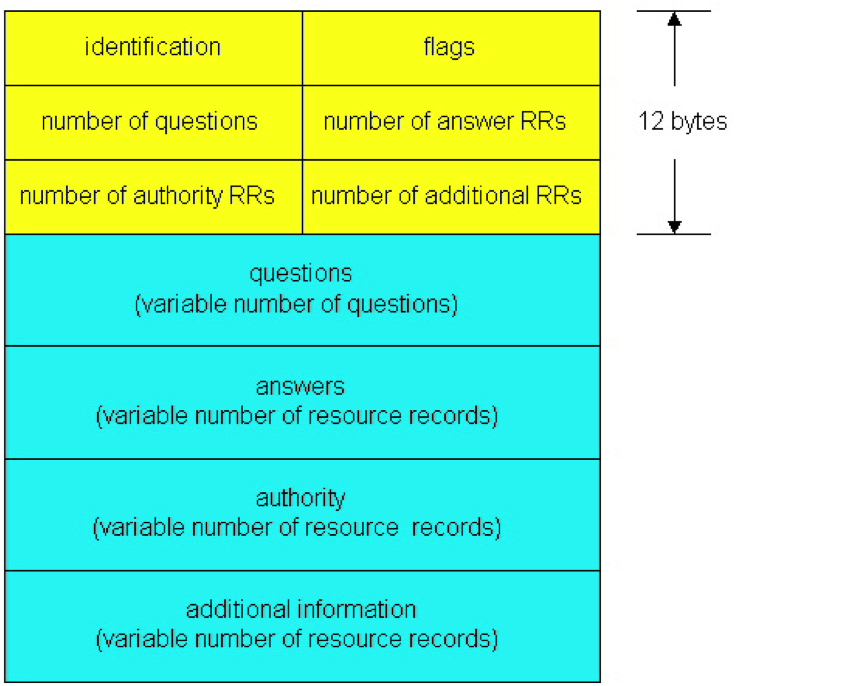
\includegraphics[width=6cm]{figs/09-dns-message.png}
  \end{center}

\end{frame}

\section{SSH}
%---------------------------------------------------------------------
\begin{frame}
  \frametitle{SSH}
  \framesubtitle{Secure Shell}
  
  Protocolo para iniciar sesiones en sevidores remotos
  \begin{itemize}
    \item Concebido como reemplazado para protocolos antiguos que usaban texto plano: {\tt rlogin}, {\tt telnet}, {\tt rsh}
    \item Diseñado para proveer comunicación seguro sobre un canal inseguro
    \item Utiliza criptografía de clave pública
    \item Diversas implementaciones. Una de las más comunes: {\tt OpenSSH}    
  \end{itemize}
\end{frame}
%---------------------------------------------------------------------
\begin{frame}
  \frametitle{SSH}
  \framesubtitle{Secure Shell}

  Aplicaciones  
  \begin{itemize}
    \item Ejecución de sesiones en servidores remotos
    \item Transferencia segura de archivos: {\tt scp}, {\tt rsync}, {\tt sftp}
    \item Ejecución de aplicaciones gráficas remotas (X forwarding)
    \item Proxy seguro (SOCKS)
    \item Montar directorios remotos de manera segura ({\tt SSHFS})
    \item Redirección de puertos a través de un canal seguro ({\em tunneling})
  \end{itemize}
\end{frame}
%---------------------------------------------------------------------
\begin{frame}
  \frametitle{SSH Tunneling}

  Utilizar un acceso {\tt ssh} para encauzar comunicación.

  Ejemplos:
  \begin{itemize}
    \item Local port forwarding
    \item Remote port forwarding
    \item Dynamic port forwarding
  \end{itemize}

\end{frame}
%---------------------------------------------------------------------
\begin{frame}
  \frametitle{SSH Tunneling}
  \framesubtitle{Local Port Forwarding}

  Problema: Deseamos acceder a un sitio, pero está bloqueado

  \begin{center}
    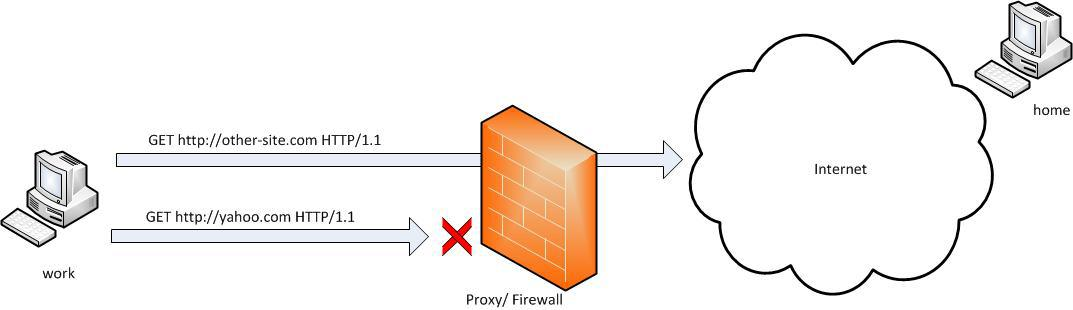
\includegraphics[width=8cm]{figs/09-sshproblem.jpg}
  \end{center}


\end{frame}
%---------------------------------------------------------------------
\begin{frame}
  \frametitle{SSH Tunneling}
  \framesubtitle{Local Port Forwarding}

  Solución, establecer un túnel a través de un servidor que tenga acceso al sitio bloqueado.
  
  \begin{center}
    {\tt ssh -L <local-port-to-listen>:<remote-host>:<remote-port>}
   
    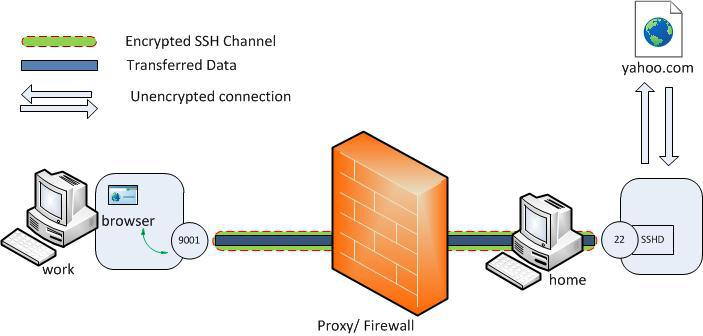
\includegraphics[width=8cm]{figs/09-sshlocal.jpg}
    
    {\tt ssh -L 9001:yahoo.com:80 home}
  \end{center}
   
   Ahora es posible conectar a {\tt http://localhost:9001}
\end{frame}
%---------------------------------------------------------------------
\begin{frame}
  \frametitle{SSH Tunneling}
  \framesubtitle{Local Port Forwarding}

  También es posible acceder a puertos bloqueados:
  \begin{center}
    {\tt ssh -L 5900:localhost:5900 home}
  \end{center}
  
  O a servidores ``prohibidos'':
  
  \begin{center}
    {\tt ssh -L 9001:banned:22 home}
   
    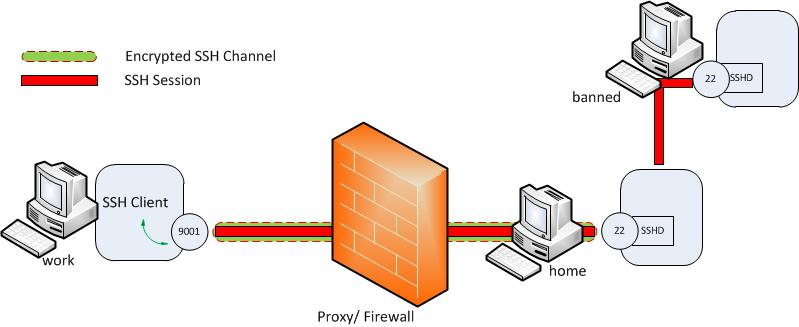
\includegraphics[width=8cm]{figs/09-sshlocalsession.jpg}
    
  \end{center}
   
   Con lo cual ahora es posible conectarse con {\tt ssh -p localhost:9001}
\end{frame}
%---------------------------------------------------------------------
\begin{frame}
  \frametitle{SSH Tunneling}
  \framesubtitle{Reverse Tunnelling}

  Problema: acceder a un sitio interno, desde afuera\footnote{Suponiendo que no tenemos una VPN, que sería una mejor solución}
  
  Solución: túnel reverso (ejecutado desde {\em work})
  \begin{center}
    {\tt ssh -R 9001:intra-site.com:80 home}
  
    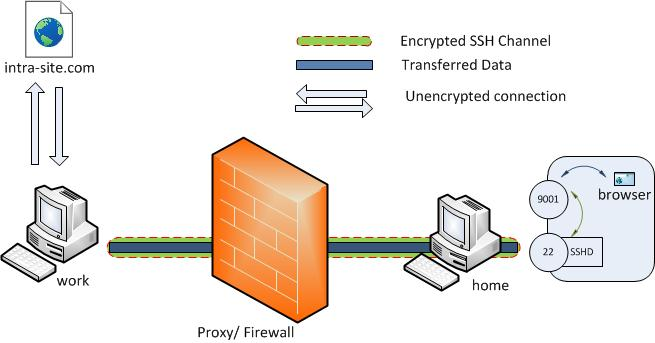
\includegraphics[width=8cm]{figs/09-sshreverse.jpg}
  \end{center}

   Ahora es posible conectar a {\tt http://localhost:9001} (desde {\em home})

\end{frame}
%---------------------------------------------------------------------
\begin{frame}
  \frametitle{SSH Tunneling}
  \framesubtitle{Dynamic Forwarding}

  Problema: acceder a un sitio interno desde afuera. {\em Reverse Tunnelling} sirve, pero es necesario
  crear un túnel para cada conexión.
  
  Solución: usar un puerto como {\em proxy}
  \begin{center}
    {\tt ssh -D 9001 home}, permite configurar un proxy SOCKS
  
    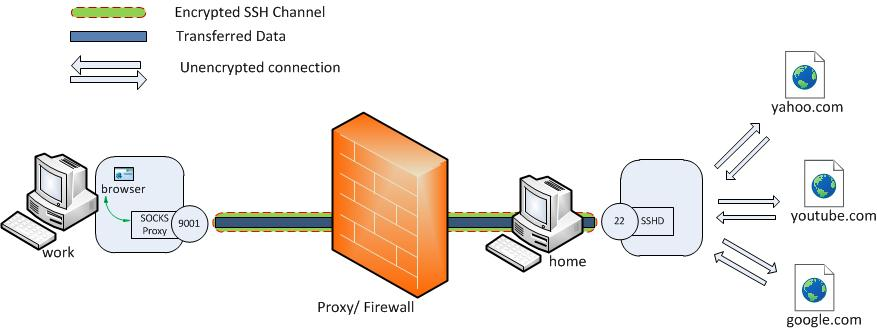
\includegraphics[width=8cm]{figs/09-sshdynamic.jpg}
  \end{center}

   Requieren configurar el navegador para conectar a un proxy SOCKS en {\tt localhost:9001}

\end{frame}
%---------------------------------------------------------------------




\end{document}